\setmainfont{Truetypewriter PolyglOTT}

\begin{titlepage}
  \begin{tikzpicture}[remember picture, overlay]
    \node[anchor=center, inner sep=0pt] at (current page.center){
      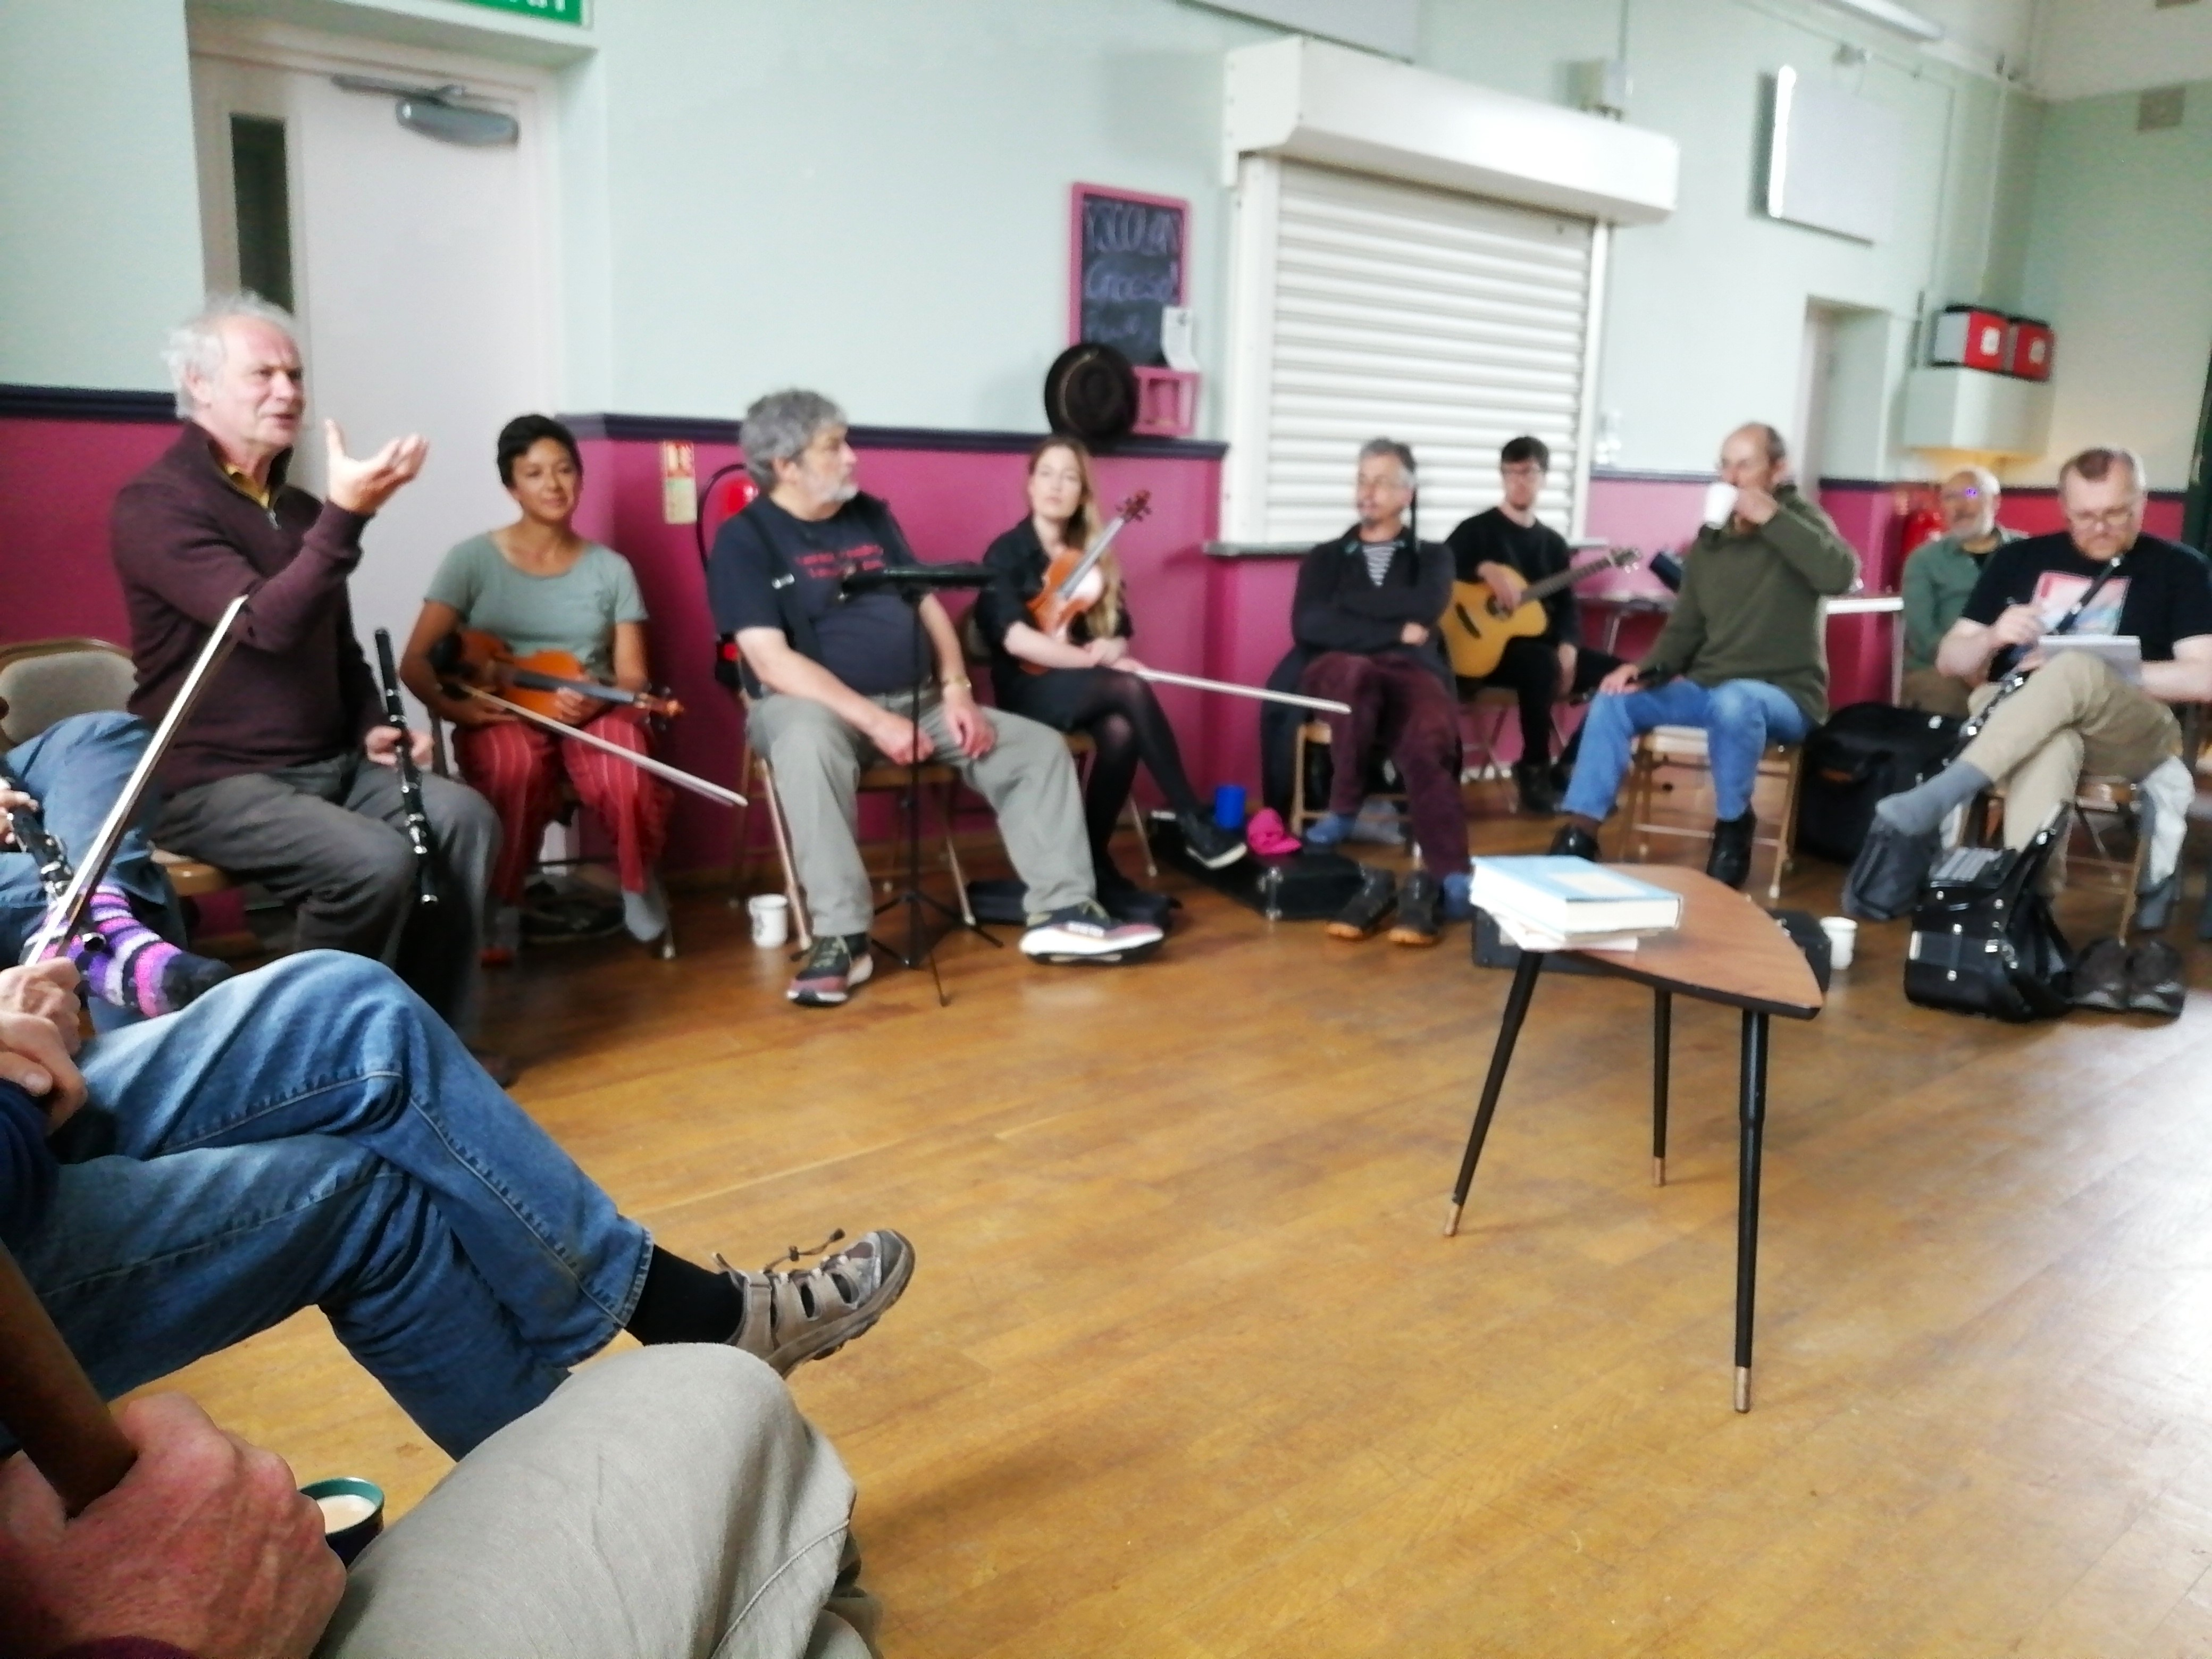
\includegraphics[
        width=\paperwidth,
        height=\paperheight
      ]{../../../assets/cover.jpg}
    };
    \node[
      fill=black,
      text=white,
      anchor=north east,
      xshift=20cm, yshift=13.5cm,
      opacity=0.7, text opacity=1
    ] at (current page.south west) {
      \fontsize{24}{48}\selectfont
      
    };

    \node[
      fill=white!20,
      anchor=south east,
      xshift=13cm, yshift=3cm,
      opacity=0.7, text opacity=1
    ] at (current page.south west) {
      \fontsize{42}{48}\selectfont
      Making the Marks
    };

    \node[
      fill=white!20,
      anchor=south east,
      xshift=16cm, yshift=2cm,
      opacity=0.7, text opacity=1
    ] at (current page.south west) {
      \fontsize{17}{24}\selectfont
      still drawing of a theoretical object
    };

    \node[
      fill=black,
      text=white,
      anchor=south east,
      xshift=20cm, yshift=1cm,
      opacity=0.7, text opacity=1
    ] at (current page.south west) {
      \fontsize{17}{24}\selectfont
      notes from Yscolan with Ceri Rhys Matthews
    };

  \end{tikzpicture}
\end{titlepage}